\chapter[Procedimientos simulaciones radiación]{Procedimientos seguidos para la realización de las simulaciones de radiación de campo cercano}\label{ch:procedimientosSimRad}

En este apéndice se detallan los pasos genéricos seguidos para la realización de las simulaciones de radiación de campo cercano y la obtención de los resultados de las potencias integradas en un respectivo rango espectral utilizando la aplicación \textbf{calculadora de campo cercano}, descrita en la sección \ref{sec:calc_campo_cercano}.

\section{Procedimientos genéricos}
Existen solo cuatro posibles casos de simulaciones de transmisión de calor por radiación de campo cercano utilizando la aplicación, estos casos son los siguientes:
\begin{itemize}
	\item Una distancia de separación y un par de materiales, uno para el emisor y otro para el receptor.
	\item Rango de distancias de separación y un par de materiales.
	\item Una distancia de separación y varias combinaciones de materiales.
	\item Rango de distancias de separación y varias combinaciones de materiales.
\end{itemize}
Los procedimientos para la realización de las simulaciones de transmisión de calor por radiación de campo cercano siguen el mismo orden de ejecución genérico. Estos procedimientos son:
\begin{itemize}
	\item Selección de la temperatura del emisor, que para este trabajo se mantiene a 1073K (800\textdegree C).
	\item Selección de las combinaciones de materiales a simular.
	\item Selección del rango de distancias a simular.
	\item Hacer clic sobre el botón \textbf{Calculate}.
\end{itemize}
%%%%%%%%%%%%%%%%%%%%%%%%%%%%%%%%%%%%%%%%%%%%%%%%%%%%%%%%%%5
%%%%%%%%%%%%%%%%%%%%%%%%%%%%%%%%%%%%%%%%%%%%%%%%%%%%%%%%%%
\section{Distancia fija y un par de materiales}
Se siguen los siguientes pasos:
\begin{enumerate}
	\item Seleccionar el material de la placa superior en \textbf{Superior plate} (figura \ref{unParMat}). 
	\item Seleccionar el material de la placa inferior en \textbf{Inferior plate}.
	\item Seleccionar la distancia (figura \ref{unaDistancia}). 
%%%%%
\begin{figure}[H]
\centering
\begin{subfigure}[b]{.48\textwidth}
	\centering
		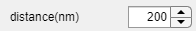
\includegraphics{figuras/unaDistancia.PNG}
	\caption{ }
	\label{unaDistancia}
\end{subfigure} \hfill
\begin{subfigure}[b]{.48\textwidth}
	\centering
		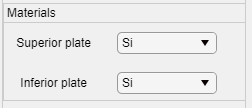
\includegraphics{figuras/unParMat.PNG}
		\caption{ }
	\label{unParMat}
\end{subfigure}
\caption{Seleccionador de una distancia de separación en nanometros (\subref{unaDistancia}) y seleccionar de los materiales de emisor (Superior plate) y receptor (Inferior plate) (\subref{unParMat}) de la calculadora de campo cercano.}
\label{fig:sencillo}
\end{figure}	
	\item Hacer click sobre el botón \textbf{Calculate}.
	\item Esperar que el indicador de estado pase de \textit{Running...}, color rojo del indicador (figura \ref{fig:indicador_Running2}), a \textit{StdBy}, color verde del indicador (figura \ref{fig:indicador_StdBy2}), es decir, esperar que termine la simulación.
	\end{enumerate}
		%% figuras de estados
	\begin{figure}[H]
	\centering
	%% Figura 1
	\begin{subfigure}[b]{0.3\textwidth}
	\centering
	
\includegraphics[width=\textwidth]{figuras/Procedimiento_Simulaciones/Radiacion/estado_changed}%
	\caption{Changed}%
	\label{fig:indicador_Changed2}%
	\end{subfigure}
	\hfill
	%% Figura 2
	\begin{subfigure}[b]{0.3\textwidth}
	\centering
	
\includegraphics[width=\textwidth]{figuras/Procedimiento_Simulaciones/Radiacion/estado_running}%
	\caption{Running}%
	\label{fig:indicador_Running2}%
	\end{subfigure}
	\hfill
	%% Figura 3
	\begin{subfigure}[b]{0.3\textwidth}
	\centering
	
\includegraphics[width=0.9\textwidth]{figuras/Procedimiento_Simulaciones/Radiacion/estado_stdby}%
	\caption{StdBy}%
	\label{fig:indicador_StdBy2}%
	\end{subfigure}
	\hfill
	\caption{Indicadores del estado actual del sistema. (\subref{fig:indicador_Changed2}) Indicador del estado \textbf{Changed} o estado de cambio, se activa cuando se produce algún cambio en los datos seleccionados para simular. (\subref{fig:indicador_Running2}) Indicador del estado \textbf{Running} o corriendo, se activa cuando estando en el estado \textbf{Changed} se hace clic al botón \textbf{Calculate} y corre la simulación. (\subref{fig:indicador_StdBy2}) Indicador del estado \textbf{StdBy}, se activa cuando termina la simulación, avisando que está a la espera de algún cambio.}
	\label{fig:indicadorLED2}
	\end{figure}
	%%%%%%%%%%%%%%%%%%%%%%%%%%%%%%%%%%%%%%%%%%%%%%%%%%%%%%%%%%%%%
%%%%%%%%%%%%%%%%%%%%%%%%%%%%%%%%%%%%%%%%%%%%%%%%%%%%%%%%%%%%%%%
\section{Rango de distancias y un par de materiales}
\begin{enumerate}
	\item Seleccionar el material de la placa superior en \textbf{Superior plate} (figura \ref{unParMat}).
	\item Seleccionar el material de la placa inferior en \textbf{Inferior plate}.
	\item Hacer click sobre el checkbox \textbf{Distance Range} (figura \ref{fig:check_distances2}).
	\item Hacer click sobre el botón \textbf{set} del \textbf{Distance Range}, que produce que aparezca la ventana de la figura \ref{fig:set_distances2}.
	\item Seleccionar el rango de distancias deseado o el checkbox \textbf{Full Range}, según lo que se desee. Para este trabajo se selecciona el checkbox \textbf{Full Range}.
	\item Hacer click en \textbf{Accept} de la nueva ventana.
	\item Hacer click sobre el botón \textbf{Calculate} y esperar a que termine de ejecutarse la simulación.
\end{enumerate}
	\begin{figure}[H]%
	\begin{subfigure}[b]{0.48\textwidth}
		\centering
			
\includegraphics[width=0.6\textwidth]{figuras/Procedimiento_Simulaciones/Radiacion/check_distances2.png}
		\caption{Checkbox de distancias}
		\label{fig:check_distances2}
	\end{subfigure}
	\hfill
	\begin{subfigure}[b]{0.48\textwidth}
		\centering
			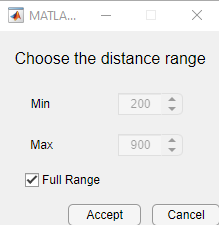
\includegraphics[width=0.6\textwidth]{figuras/Procedimiento_Simulaciones/Radiacion/set_distances_fullrange.png}
		\caption{Set de distancias}
		\label{fig:set_distances2}
	\end{subfigure}
	\caption{(\subref{fig:check_distances2}) Casilla para la selección de la opción de simular un rango de distancias. (\subref{fig:set_distances2}) Ventana para la selección del rango de distancias a simular.}%
	\label{fig:checkboxes2}%
	\end{figure}
	%%%%%%%%%%%%%%%%%%%%%%%%%%%%%%%%%%%%%%%%%%%%%%%%%%%
	%%%%%%%%%%%%%%%%%%%%%%%%%%%%%%%%%%%%%%%%%%%%%%%%%%%
	\section{Distancia fija y varios materiales}
	\begin{enumerate}
			\item Hacer click sobre el checkbox \textbf{Materials Range} (figura \ref{fig:check_materials2}).
			\item Hacer click sobre el botón \textbf{set} del \textbf{Materials Range}, que produce que aparezca la ventana de la figura \ref{fig:set_materials2}.
			\item Seleccionar los materiales para la cara superior (UpFace) (figura \ref{fig:set_materials2}).
			\item Seleccionar los materiales para la cara inferior (DownFace).
			\item Hacer clic en \textbf{Accept} de la ventana emergente.
			\item Seleccionar la distancia (figura \ref{unaDistancia}). 
			\item Hacer click sobre el botón \textbf{Calculate} y esperar a que termine de ejecutarse la simulación.
	\end{enumerate}
	%%%%%%%%%%%%%%%%%
	\begin{figure}[H]%
	\begin{subfigure}[b]{0.48\textwidth}
		\centering
			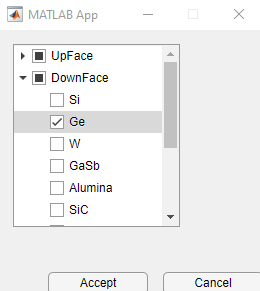
\includegraphics[width=0.6\textwidth]{figuras/Procedimiento_Simulaciones/Radiacion/set_materilas2.png}
		\caption{Set de materiales}
		\label{fig:set_materials2}
	\end{subfigure}\hfill
		\begin{subfigure}[b]{0.48\textwidth}
		\centering
			
\includegraphics[width=0.6\textwidth]{figuras/Procedimiento_Simulaciones/Radiacion/check_materials2.png}
		\caption{Checkbox de materiales}
		\label{fig:check_materials2}
	\end{subfigure}
	\caption{(\subref{fig:set_materials2}) Ventana para la selección de las combinaciones de materiales a simula, siendo \textbf{UpFace} el emisor y \textbf{DownFace} la célula.	(\subref{fig:check_materials2}) Casilla para la selección de la opción de simular una combinación de materiales.}%
	\label{fig:sets2}%
	\end{figure}	
	%%%%%%%%%%%%%%%%%%%%%%%%%%%%%%%%%%%%%%%%%%%%%%%%%%%%
	%%%%%%%%%%%%%%%%%%%%%%%%%%%%%%%%%%%%%%%%%%%%%%%%%%%%
\section{Rango de materiales y varios materiales}
\begin{enumerate}
			\item Hacer click sobre el checkbox \textbf{Materials Range} (figura \ref{fig:check_materials2}).
			\item Hacer click sobre el checkbox \textbf{Distance Range} (figura \ref{fig:check_distances2}).
			%% MATERIALS
			\item Hacer click sobre el botón \textbf{set} del \textbf{Materials Range}, que produce que aparezca la ventana de la figura \ref{fig:set_materials2}.
			\item Seleccionar los materiales para la cara superior (UpFace) (figura \ref{fig:set_materials2}).
			\item Seleccionar los materiales para la cara inferior (DownFace).
			\item Hacer clic en \textbf{Accept} de la ventana emergente.
			%%%% DISTANCE
			\item Hacer click sobre el botón \textbf{set} del \textbf{Distance Range}, que produce que aparezca la ventana de la figura \ref{fig:set_distances2}.
			\item Seleccionar el rango de distancias deseado o el checkbox \textbf{Full Range}, según lo que se desee. Para este trabajo se selecciona el checkbox \textbf{Full Range}.
			\item Hacer click en \textbf{Accept} de la nueva ventana.
			\item Hacer click sobre el botón \textbf{Calculate} y esperar a que termine de ejecutarse la simulación.
\end{enumerate}

\chapter{Acrónimos}

\let\cleardoublepage\clearpage
\glsaddall
\cleardoublepage
\printglossary[type=\acronymtype,title=Acr\'{o}nimos]
%\printnoidxglossary[type=\acronymtype,title=Acr\'{o}nimos]%,sort=use]%[type=\acronymtype]

%\printglossary